\documentclass[11pt]{amsart}
\usepackage{geometry}                % See geometry.pdf to learn the layout options. There are lots.
\geometry{letterpaper}                   % ... or a4paper or a5paper or ... 
\usepackage[parfill]{parskip}    % Activate to begin paragraphs with an empty line rather than an indent
\usepackage{graphicx}
\usepackage{amssymb}
\usepackage{epstopdf}
\usepackage{cite}
\usepackage{graphics}
\usepackage[linesnumbered,vlined,algoruled]{algorithm2e}
\DeclareMathOperator*{\argmax}{arg\,max}
\DeclareMathOperator{\argmin}{arg\,min}

\usepackage{amsmath,amssymb}  % Better maths support & more symbols
\usepackage{bm}  % Define \bm{} to use bold math fonts

\usepackage{pdfsync}  % enable tex source and pdf output syncronicity
\DeclareGraphicsRule{.tif}{png}{.png}{`convert #1 `dirname #1`/`basename #1 .tif`.png}

\title{K-means Clustering at Scale}
\author{Ted Dunning}
%\date{}                                           % Activate to display a given date or no date
\begin{document}
\begin{abstract}
Implementing a $k$-means algorithm at scale using map-reduce techniques can be difficult using Hadoop due to program invocation overhead and total I/O requirements.  There have been efforts to attack the program invocation cost of Hadoop by having a single program invocation run multiple iterations by using an {\em all-reduce} primitive or by using an in-memory system like Spark.  Neither of these alternatives addresses the cost of reading large data sets and the work described here would accelerate both of these alternatives.

This paper describes an approach for large scale clustering based on the streaming $k$-means algorithm.  The implementation described here requires only a single pass over the input data which results in multiple order of magnitude throughput improvement.  Even if process invocation is ignored, avoiding multiple passes over the input has major impacts on running time because simply reading a large data set is typically the dominant cost in large-scale computations.
\end{abstract}
\maketitle
\section{Introduction and Background}

The $k$-means algorithm is a special case of the general EM framework which can be used to solve for a mixture distribution that approximates the distribution of observed data.  The commonly used algorithm due to Lloyd\cite{k-means} involves assignment of observations to a nearest cluster (the E step) followed by recomputation of cluster positions by averaging the observations assigned to each cluster (the M step).
The conceptual and implementation simplicity of Lloyd's algorithm have made it extremely popular.  Moreover, EM-based algorithms like this are easily encoded as multiple map-reduce steps in which the E step is computed in a map function and the M step is computed in combiner and reducer functions.

Many variations have been developed which alter the initial values chosen for the cluster centroids.  Propitious initialization can substantially improve the quality of the resulting clusters and may decrease the number of iterations required to converge.  Other algorithms try to address the choice of the number of clusters.  Still others extend the basic algorithm to avoid hard assignment to clusters through the use of fuzzy logic, non-deterministic assignment or a full Bayesian treatment.  The Apache Mahout library\cite{mahout}
 contains implementations of standard $k$-means, fuzzy $k$-means, a canopy clustering implementation as well as a variety of more or less Bayesian mixture distribution algorithms.  

Most of these variants still require multiple passes through the data and none address the problems of having to run multiple map-reduce iterations or the cost of reading the data multiple times.

Recently, a number of algorithms have been developed which address the iterative nature of $k$-means clustering by radically increasing the number of clusters used.  These location of and number of points in these clusters can be taken as a surrogate for the original data distribution and a weighted $k$-means algorithm can be applied to the clusters themselves to derive a clustering for the original data.  

The number of clusters to be clustered in this secondary step is large compared to the final number of clusters but is quite small compared to the original number of observations.  As such, the final clustering step can generally be done in memory and contributes negligible time to the overall process.  In some cases such as nearest neighbor search, having a large number of clusters is entirely acceptable and the post-clustering step is unnecessary.  One of these new clustering algorithms, streaming $k$-means\cite{DBLP:conf/nips/ShindlerWM11}, is particularly simple and provides good theoretical convergence guarantees if enough intermediate clusters are used.  Happily, the number of intermediate clusters required only grows according to $O(\log n)$ where $n$ is the number of observations in the original data.  Practically speaking, the size of memory required by the final clustering step is a non-issue with modern computers which typically have gigabytes of available memory.

The basic outline of the streaming $k$-means algorithm described in this paper consists of a clustering algorithm that is presented with a stream of observations.  The incoming observations are assigned to a nearby cluster or are used as the basis of a new cluster.  This choice is made stochastically according to how distance to the nearby cluster compares to an adaptive scale parameter.  Over time, the number of clusters eventually grows to a limit based on memory size or theoretical considerations.  When this happens, the clusters themselves are passed through an instance of the same on-line clustering step in order to combine nearby clusters and so decrease the number of clusters.  If the number of clusters is not substantially decreased by this recursive clustering, then the scale parameter is increased so that subsequent observations are more likely to adhere to existing clusters and so that the recursive clustering is more likely to be effective at decreasing the number of clusters.

For the map-reduce implementation, this basic algorithm is done independently on disjoint portions of the data in the map phase.  Each mapper independently finds a large number of clusters appropriate for the data it sees.  These centroids are passed to the reduce function which uses the basic algorithm to decrease the number of clusters to the desired number.

Having a large number of clusters to search for each observation can make finding the nearest cluster expensive if brute force search is used.  To avoid this search becoming a bottle neck, the implementation described here uses a projection search.  In this projection search, several random vectors are selected.  Associated with each random vector is a tree that contains references to all of the cluster centroids ordered according to the projection of the cluster centroid in the direction of the random vector.  With even a small number of projections, the nearest cluster can be found with high probability even though only a few vectors are actually tested.

\section{Implementation}
\subsection{Initializing the Scale Factor}
In the original description of the streaming $k$-means algorithm, the scale factor was initialized based on the number of data points.  This has two problems.  First, if we only want to make a single pass over the data, then we won't know the total number of data points until after we are done clustering.  Secondly, initializing the scale factor based on the number of points presumes that the data has been normalized which also requires an additional pass over the data.

Neither of these issues is inherent.  All that is necessary is that the scale factor be initially set small enough so that we get enough clusters.  In this implementation, the way that this is done is to take a small sample of points and set the scale factor to the smallest distance between any of the sample points.

\begin{algorithm}[H]
\SetNoFillComment
\KwIn{Sample of $m$ observations $\left \lbrace x_1 \ldots x_m \right \rbrace$ }
\KwOut{Scale factor $f$}
\ForEach{$i \in 1 \ldots m$}{
\ForEach{$i \in 1 \ldots m$}{
  $f = \min(f, | x_i - x_j |)$
}
}
\Return $f$
\caption{Function {\tt initialCutoff} for finding an initial distance cutoff}
\end{algorithm}

\subsection{Projection Search for Nearest Cluster}
Finding the nearest cluster is a key operation in the streaming $k$-means algorithm just as it is in other $k$-means algorithms.  The importance of doing this efficiently is magnified by the fact that streaming $k$-means must search many more than $k$ clusters.  In order to decrease these costs, the implementation described here uses a random projection to reduce the problem of finding a nearby cluster to a one-dimensional search.  Such a projection search does not guarantee that the nearest cluster is found even if several candidates with a short projected distance are examined.  In order to increase the chance of finding the closest cluster, the results of several projection searches can be combined. 

In Java, built-in {\tt TreeSet} provides the necessary mechanics for this search in the form of the {\tt headSet} and {\tt tailSet} methods.  These methods are defined as
\[
\mathtt{headSet}(S, k) = \lambda(S,k). \left\lbrace s_i \in S \mid s_i < k \right\rbrace
\]
\[
\mathtt{tailSet}(S, k) = \lambda (S,k). \left\lbrace s_i \in S \mid s_i \ge k \right\rbrace
\]
The algorithm for indexing a set of vectors is

\begin{algorithm}[H]
\SetNoFillComment
\KwIn{observations $\left \lbrace x_1 \ldots x_n \right \rbrace$ }
\KwOut{projection vectors, $v_1 \ldots v_m$, tree sets $s_1 \ldots s_m$}
\ForEach{$j \in 1 \ldots m$}{
$v_j \sim \mathrm {MultiNormal}(0, \mathrm I) $ \\
$s_j$ = {\tt new TreeSet()}
}
\ForEach{$i \in 1 \ldots n$}{
\ForEach{$j \in 1 \ldots m$}{
   $s_j = s_j \cup (x_i \cdot v_j, x_i)$
}
}
\caption{Projection search indexing}
\end{algorithm}

The algorithm for searching a projection search like this is also quite simple

\begin{algorithm}[H]
\SetNoFillComment
\KwIn{query vector $q$, projection vectors, $v_1 \ldots v_m$, tree sets $s_1 \ldots s_m$ }
\KwOut{approximation of the $k$ vectors nearest to $q$ }
candidate set $r = \lbrace \rbrace$ \\
\ForEach{$j \in 1 \ldots m$}{
   $z = v_j \cdot q$ \\
   $r = r \cup \mathtt{tailSet} (s_j, z)[1 \ldots l]  \cup \mathtt{reverse} ( \mathtt{headSet}(z))[1 \ldots l]$
}
\Return { $\mathtt{sort}(r, \lambda u. |u-q|)[1 \ldots k] $}
\caption{Projection search \label{projection-search}}
\end{algorithm}

The idea here is that the set $r$ is constructed out of the elements that are less than or equal to $l$ positions before or after the position the query vector would have in the set of vectors if they are ordered after projecting onto each of the $v_j$.  Any vector that is near $q$ must also be near $q$ after projecting onto each of the $v_j$.  In the projection, however, a number of other vectors not near $q$ may also appear nearby.  If $l$ is large enough and the number of projections $m$ is large enough, then the list returned by projection search will be correct.  What is more interesting is that for substantially small values of $l$ and $m$, the return list will have high overlap with the correct list.

For the purposes of streaming $k$-means, only the nearest cluster is required and it isn't even necessary that precisely the nearest cluster be returned every time.  The ratio of the distance to the nearest returned item to the distance to the true nearest neighbor is also interesting.  For a given data distribution, both the probability of correct return and this ratio depend on the dimension of the problem, the search size $l$ and the number of projections $m$.  

Figure \ref{projection-probability} shows how the probability of finding the nearest cluster declines with increasing dimension for a search 10,000 points that have a unit normal distribution.  It should be noted that even with 500 dimensions, the probability of finding the nearest cluster is high enough that combining 20 projections provides a roughly 80\% chance of finding the nearest cluster.   The theoretical bounds on the streaming $k$-means algorithm given in \cite{DBLP:conf/nips/ShindlerWM11} suggest that high accuracy in finding the nearest clustering during the clustering algorithm is not necessary for achieving high clustering quality, but that situation is different when doing nearest neighbor search using a $k$-means clustering as a component of the search.  Using the same projection search during assignment of points to centroids as during search may help with this since errors in assignment to clusters may be correlated.
\begin{figure}[htbp]
\begin{center}
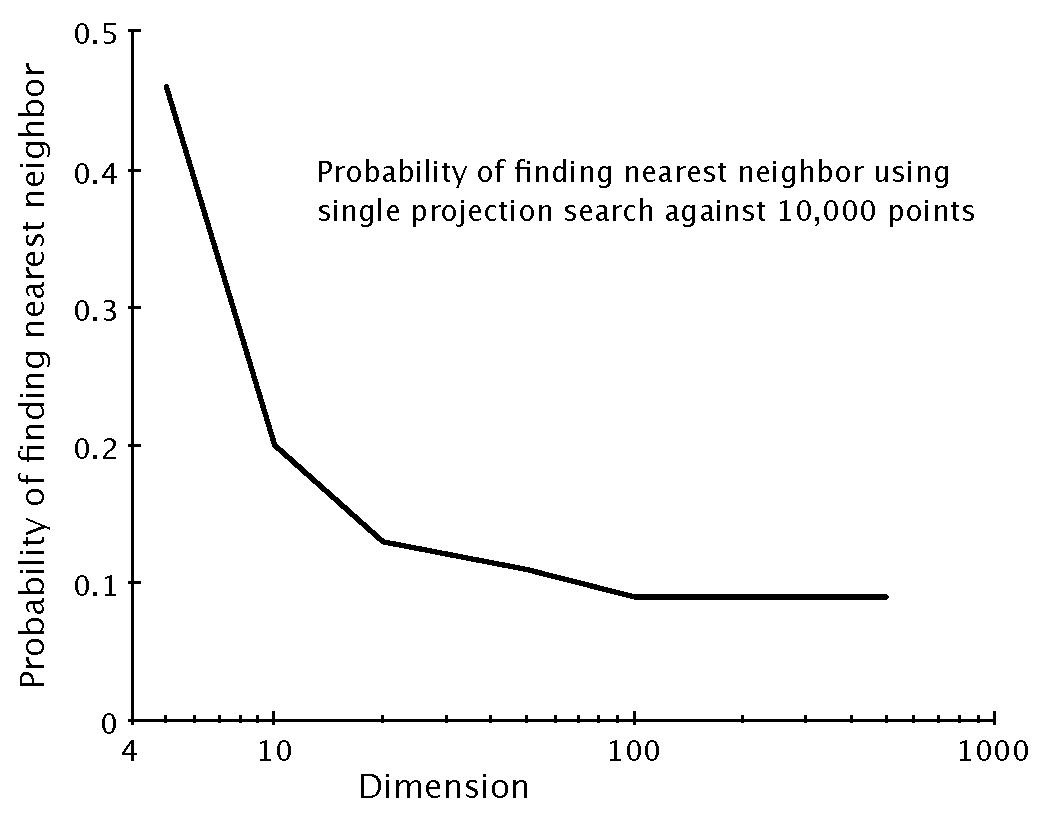
\includegraphics[width=4in]{projection-probability.pdf}
\caption{{\bf The probability of finding the nearest cluster using a single projection search declines with increasing dimension}}
\label{projection-probability}
\end{center}
\end{figure}
On the limited number of real data sets that we have examined we have observed that projection search seems to find the nearest neighbor more accurately than the experiments shown in Figure \ref{projection-probability} would indicate.
\subsection{Sequential Clustering Algorithm}
The sequential form of the streaming $k$-means algorithm uses the function {\tt cluster} which passes over the observations $x_1 \ldots x_n$  to form a set of weighted cluster centroids $C = \left\lbrace c_1 \ldots c_k\right\rbrace$.  The observations are assumed to be structures containing a weight $w$ and a vector position $r$.  Normally, the weights for all observations is set to $1$.  As the observations are processed, the size of the set of centroids found so far will increase so that it will eventually exceed a limit $\kappa$ which is either set based on the number of points seen so far or a user-provided target.  When the size exceeds $\kappa$, the centroids themselves are clustered using the same logic but further recursion is prevented.  If the recursive clustering is successful in substantially decreasing the number of centroids, then processing continues.  If not, the distance cutoff is increased by a factor $\beta$ which is typically set to a value of $1.25$ to $1.5$.  Increasing the distance cutoff $f$ makes it less likely that observations will be added to $C$ as new clusters and thus makes it take longer for $|C|$ to reach $\kappa$.  Increasing $f$ also makes it more likely that the recursive clustering will substantially decrease the number of centroids.

\begin{algorithm}[H]
\SetNoFillComment
\KwIn{observations $x_1 \ldots x_n$, initial distance cutoff $f_0$, target number of centroids $\kappa_0$, recursion depth $d$ }
\KwOut{distance cutoff $f$, weighted centroids $C = \left \lbrace (w_i, c_i)\mid i=1\ldots k\right \rbrace$} 
$C = \left \lbrace x_1 \right \rbrace$ \\
$f = f_0$ \\
$n = x_1[w]$ \\
\ForEach{$i \in 2 \ldots n$} {
   $n \Leftarrow n + x_i[w]$ \\
   $c = \argmin_{c \in C} \left | c[r] - x_i \right |$\\
   $d = |c-x_i|$ \\
   $u \sim \mathrm{Uniform}(0,1)$\\
   \If {$u < d/f$} {
       $C \Leftarrow C \cup  x_i$ 
   }
   \Else {
       $c[r] \Leftarrow\frac{c[w] c[r] + x_i[w] x_i[r]} { c[w] + x_i[w]} $\\
       $c[w] \Leftarrow c[w] + x_i[w]$
   }
   $\kappa \Leftarrow \min(\kappa_0, 10 \log n)$ \\
   \If {$|C| > \kappa$ and $d = 0$} {
      $k = |C|$ \\
      $C \Leftarrow \mathtt {cluster}( C, f, \kappa, d+1 )$ \\
      \If {not $|C| \ll k$} {
          $ f \Leftarrow \beta f$
      }
   }
}
\Return {$f, C $}
\caption{The {\tt cluster} function}
\end{algorithm}

The search for the nearest cluster is implemented using the projection search defined above as Algorithm \ref{projection-search}.

The clustering algorithm as stated here has been changed from the original streaming $k$-means in several respects.  These change include the way that the distance cutoff is only conditionally increased and the way that $\kappa$ depends on the points seen so far rather than on the total number of points.  Both changes seem to have a positive impact in practice and there seems at first glance to be no real difference in the theoretical bounds on the algorithm due to these changes.
\subsection{Map-reduce Implementation}

The map-reduce implementation of streaming $k$-means is straightforward.  The first step is computation of an initial cutoff using a sample of points from throughout the input sequence.  Then the input data is split and each split is passed to a mapper that consists of an instance of the streaming $k$-means algorithm.  The results of clustering each split are all passed to a single reducer uses the streaming $k$-means function to combine the clusters as needed.

\begin{algorithm}[H]
\SetNoFillComment
\KwIn{distance cutoffs and centroids from each mapper $\lbrace (f_1, C_1) \ldots (f_r, C_r) \rbrace$, 
target number of centroids $\kappa_0$ }
\KwOut{weighted centroids $ (w_i, c_i) $ where $i=1\ldots k$} 
$f = \min_i f_i$ \\
$n = \sum_i C_i[w]$\\
$\kappa = \max\left(\kappa_0, 10 \log n \right)$\\
\Return $ \mathtt {cluster}( \bigcup_i C_i, f, \kappa, 0)$\\
\caption{The {\tt ClusterReducer} function}
\end{algorithm}
\section{Results}

\subsection{Single Core and Multi-core Speeds}

Figure \ref{threaded-timing-16-core} shows how a single-threaded implementation of streaming $k$-means compares with a multi-threaded implementation when run on a 16 core machine.  This test used 1 million samples of normally distributed 30-dimensional random data.  

The threaded implementation exhibits  overhead relative to the single-threaded implementation as evidenced by the relative performance of the two implementations with a single thread.  Adding more cores provides nearly perfect scaling of run time up to 14 cores.  The limited improvement beyond this point is probably due to the fact that the input is always split into exactly 36 segments and when the number of threads is large, load balancing suffers.  
\begin{figure}[htbp]
\begin{center}
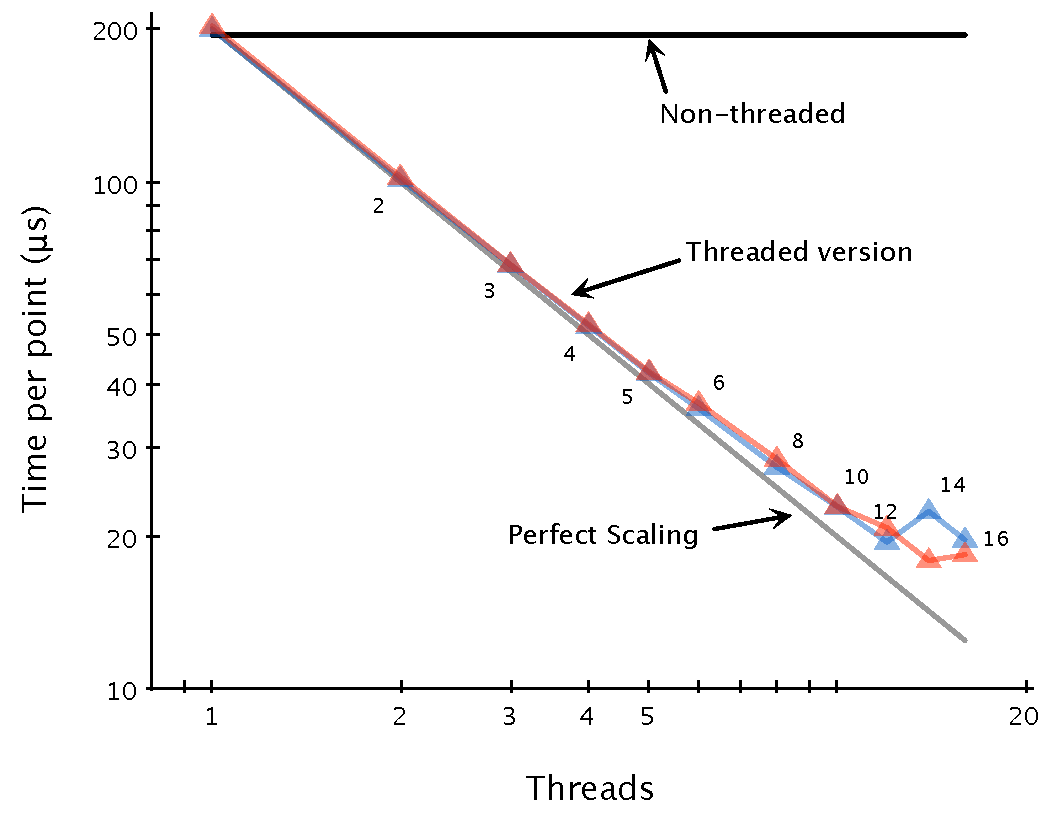
\includegraphics[width=4in]{thread-timing-16-core-1M.pdf}
\caption{{\bf The threaded version can make better use of a machine than the unthreaded version}}
\label{threaded-timing-16-core}
\end{center}
\end{figure}
\subsection{Map-reduce Speed}
\subsection{Clustering Quality}

\section{Source Code and Resources}
Java implementations of the algorithms described here are available \cite{github/knn} and is likely to be part of the Apache Mahout package starting with the 0.8 release.

The package includes a considerable amount of software for generating test distributions and doing $k$-nearest neighbor searches using a variety of algorithms which are described elsewhere.  The key class of interest is {\tt StreamingKmeans} which is in the {\tt knn.means} package under {\tt org.apache.mahout}.  This class depends on the {\tt ProjectionSearch} class in the {\tt knn.search} package.  Test classes are provided which give a sense of the possible API.
\bibliography{refs}{}
\bibliographystyle{alpha}
\end{document}  